\documentclass[12pt]{article}
\usepackage{amssymb}
\usepackage{amsmath}
\usepackage{tikz}
\usetikzlibrary{decorations.markings}

\begin{document}

			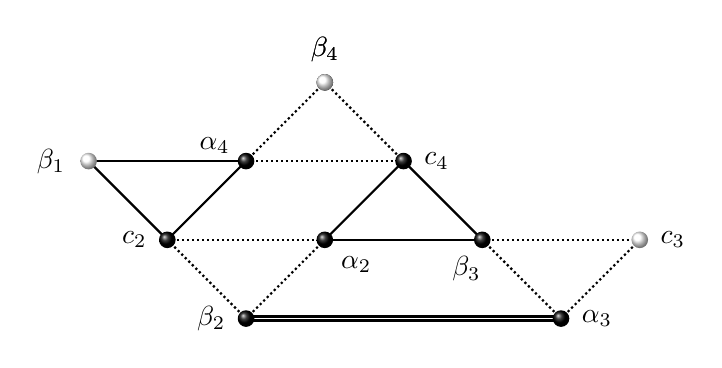
\begin{tikzpicture}[x=2cm,y=0.5cm,scale=1]
			\draw[thick] (-2,2) -- (-1,2);%beta1---alpha4
			\draw[densely dotted, thick] (-1,2) -- (0,2);%alpha4---c4

			\draw[densely dotted, thick]  (-0.5,4) -- (0,2);%beta4---alpha4
			 \draw[densely dotted, thick]  (-0.5,4) -- (-1,2);%beta4---alpha4 (error -> c4?)

			 \draw[densely dotted, thick]  (-1.5,0) -- (-0.5,0);%c2---alpha2
			\draw[densely dotted, thick]  (-0.5,0) -- (-1,-2);%alpha2---beta2
			\draw[densely dotted, thick]  (-1.5,0) -- (-1,-2);%c2---beta2

			 \draw[thick]  (0,2) -- (-0.5,0);%c4---alpha2
			\draw[thick]  (-0.5,0) -- (0.5,0);%alpha2---beta3
			\draw[thick]  (0,2) -- (0.5,0);%c4---beta3

			 \draw[thick]  (-2,2) -- (-1.5,0);%beta1---c2
			\draw[thick]  (-1.5,0) -- (-1,2);%c2---alpha2

			\draw[densely dotted, thick]  (0.5,0) -- (1.5,0);%beta3---c3
			\draw[densely dotted, thick]  (1.5,0) -- (1,-2);%c3---alpha3
			\draw[densely dotted, thick]  (0.5,0) -- (1,-2);%beta3---alpha3

            \draw[thick] (-1,-1.95) -- (1,-1.95);
            \draw[thick] (-1,-2.05) -- (1,-2.05);
			\node[above=4pt] (beta4) at (-0.5,4) {$\beta_4$};
			\shade [ball color=black] (-0.5,4) circle (3pt);

			\node [left=5pt] (beta1) at (-2,2) {$\beta_1$};
			\shade [ball color=white] (-2,2) circle (3pt);

			\node[=5pt](alpha4) at (-1.2,2.4) {$\alpha_4$};
			\shade[ball color=black] (-1,2) circle (3pt);

			\node[right=4pt] (c4) at (0,2) {$c_4$};
			\shade [ball color=black] (0,2) circle (3pt);

			\node[left=4pt] (c2) at (-1.5,0) {$c_2$};
			\shade [ball color=black] (-1.5,0) circle (3pt);

			\node[below=4pt] (alpha2) at (-0.3,0.1) {$\alpha_2$};
			\shade [ball color=black] (-0.5,0) circle (3pt);

			\node[below=4pt] (beta3) at (0.4,0.1) {$\beta_3$};
			\shade [ball color=black] (0.5,0) circle (3pt);

			\node[right=4pt] (c3) at (1.5,0) {$c_3$};
			\shade [ball color=white] (1.5,0) circle (3pt);

			\node[left=4pt] (beta2) at (-1,-2) {$\beta_2$};
			\shade [ball color=black] (-1,-2) circle (3pt);

			\node[right=4pt] (alpha3) at (1,-2) {$\alpha_3$};
			\shade [ball color=black] (1,-2) circle (3pt);

			\node[above=4pt] (beta4) at (-0.5,4) {$\beta_4$};
			\shade [ball color=white] (-0.5,4) circle (3pt);
		\end{tikzpicture}

\end{document}